% Use only LaTeX2e, calling the article.cls class and 12-point type.

\documentclass[twocolumn,showpacs,twoside,10pt,prl]{revtex4}
\usepackage{graphicx}
\usepackage{epsfig}
\usepackage{epsf}
\usepackage{amssymb}
\usepackage{amsmath}
\usepackage{amsthm}
\usepackage{multirow}
\usepackage{hyperref}

\newcommand{\bra}[1]{\langle #1|}
\newcommand{\ket}[1]{|#1\rangle}

\newcommand{\be}{\begin{equation}}
\newcommand{\ee}{\end{equation}}
\newcommand{\bea}{\begin{eqnarray}}
\newcommand{\eea}{\end{eqnarray}}
\newcommand{\Fig}[1]{Fig.\,\ref{#1}}
\newcommand{\Eq}[1]{Eq.\,(\ref{#1})}
\newcommand{\la}{\langle}
\newcommand{\ra}{\rangle}
\newcommand{\nl}{\nonumber \\}
\usepackage[usenames]{color}
\definecolor{Red}{rgb}{1,0,0}
\definecolor{Blue}{rgb}{0,0,1}





%%%%%%%%%%%%%%%%% END OF PREAMBLE %%%%%%%%%%%%%%%%



\begin{document}

% Include your paper's title here
\title{Supplementary Information for ``Simulation of Chemical Isomerization Reaction Dynamics on an NMR Quantum Simulator"}
\author{Dawei Lu$^{1}$}
\author{Nanyang Xu$^{1}$}
\author{Ruixue Xu$^{1}$}
\author{Hongwei Chen$^{1}$}
\author{Jiangbin Gong$^{2,3}$}
\author{Xinhua Peng$^{1}$}
\author{Jiangfeng Du$^{1}$}
\email{djf@ustc.edu.cn}


\affiliation{$^{1}$Hefei National Laboratory for Physical Sciences at
Microscale and Department of Modern Physics, University of Science
and Technology of China, Hefei, Anhui, 230026, China}
\affiliation{$^{2}$Department of Physics and Centre for
Computational Science and Engineering, National
University of Singapore, 117542, Republic of
Singapore}
\affiliation{$^{3}$NUS Graduate School for Integrative
Sciences and Engineering, 117597,
Republic of Singapore}


\pacs{03.67.Lx, 07.57.Pt, 42.50.Dv, 76.60.-k}
\maketitle




\subsection*{BACKGROUND ON QUANTUM DYNAMICS SIMULATION}



Let us start with the Schr\"{o}dinger equation:
\be
 i\hbar \dot\psi(t)=  H(t)\psi(t).
\ee
Its formal solution can be written as
\be
   \psi(t)=   U(t,t_0)\psi(t_0),
\ee
where the quantum propagator $U(t,t_0)$ is a unitary operator and is given by
\be
     U(t,t_0)={\cal T}\exp\left[-\frac{i}{\hbar}
  \int_{t_0}^t\!\!d\tau\,   H(\tau)\right],
\ee
with ${\cal T}$ being the time ordering operator.  There are a number of established numerical methods for propagating the Schr\"{o}dinger equation,
such as Feynman's path integral formalism \cite{Feynman2},
the split-operator method \cite{Feit2} and the Chebychev polynomial method \cite{Kosloff,Zhangbook2}, etc.  For our purpose here we adopt the split-operator method.

The propagator $U(t,t_0)$  satisfies
\be
     U(t,t_0)=   U(t,t_{N-1})   U(t_{N-1},t_{N-2})\cdots\cdots   U(t_1,t_0)\,,
\ee
where, for example, the intermediate time points can be equally spaced with $t_m=m\delta t+t_0$.
For one of such a small time interval, e.g., from $t_{m-1}$ to $t_{m}=t_{m-1}+\delta t$, we have
\begin{eqnarray}
     U(t_{m},t_{m-1})& = &{\cal T} \exp\left[-\frac{i}{\hbar}
  \int_{t_{m-1}}^{t_m}\!\!d\tau\,   H(\tau)\right] \nonumber \\
  &\approx & \exp\left[-\frac{i}{\hbar}
  \int_{t_{m-1}}^{t_m}\!\!d\tau\,   H(\tau)\right],
\end{eqnarray}
where terms of the order $(\delta t)^3$ or higher are neglected.  For sufficiently small $\delta t$,
the integral in the above equation can be further carried out by a midpoint rule, leading to
\begin{eqnarray}
     U(t_{m},t_{m-1})\approx \exp\left[-\frac{i}{\hbar} H(t_{m-1}+\delta t/2) \delta t\right].
     \label{someq}
\end{eqnarray}
This integration step has an error of the order of $(\delta t)^2$, which is still acceptable if the total evolution time
is not large.
Next we separate the total Hamiltonian into two parts:
\be
     H(t)=   H_0(t)+   H'(t).
\ee
For example, $H_0(t)$ is the kinetic energy part of the total Hamiltonian and $H'(t)$ represents the potential energy part.  In general
$H_0(t)$ and $H'(t)$ do not commute with each other.
The split-operator scheme \cite{Feit2}  applied to Eq. (\ref{someq}) then leads to
\begin{eqnarray}
  {U}(t_m,t_{m-1}) & \approx &
   e^{-\frac{i}{\hbar}   H' (t_{m-1}+\delta t/2)    \delta t/2}
   e^{-\frac{i}{\hbar}   H_0  (t_{m-1}+\delta t/2)  \delta t  }  \nonumber \\
  & & \times  e^{-\frac{i}{\hbar}   H' (t_{m-1}+\delta t/2)             \delta t/2}.
 \label{sop}
\end{eqnarray}
The small error of this operator splitting step arises from the nonzero commutator between
$ H_0(t)$ and $H'(t)$, which is at least of the order of $(\delta t)^3$.  The advantage of
the split-operator method is that each step represents a unitary evolution and each exponential in Eq. (\ref{sop}) can take a diagonal form
in either the position or the momentum representation.
  The error of this operator splitting step
is in general smaller than that induced by the aforementioned midpoint rule integration in
Eq. (\ref{someq}). Because in our work the total duration of the
simulated chemical reaction is short, the above low-order approach already has a great performance.
If long-time simulations with preferably larger time steps are needed in a quantum simulation,
then one may use even higher-order split-operator techniques for explicitly time-dependent Hamiltonians \cite{bandrauk,zhu}.


\subsection*{EXPERIMENTAL IMPLEMENTATION}

The experiment consists of three steps: (a) Initial state preparation, which is to prepare the ground state $\left\vert \phi_{0} \right\rangle$ of the bare Hamiltonian $T+ {V}$ (representing the reactant state); (b) 25 discrete steps of dynamical evolution to simulate the actual continuous chemical reaction dynamics; (c) Measurement of the overlaps $C(\left\vert \psi(t_j) \right\rangle,\left\vert \phi_{0} \right\rangle)=| \la\phi_0|\psi(t_j)\ra |^2$ and $C(\left\vert \psi(t_j) \right\rangle,\left\vert \phi_{1} \right\rangle)=| \la\phi_1|\psi(t_j)\ra |^2$ at $t_j=j\delta t$, which is to show the transformation between the reactant and product states.

\subsubsection*{\textbf{A. Initial State Preparation}}


To prepare the ground state $\left\vert \phi_{0} \right\rangle$, firstly we need to create a pseudo-pure state (PPS) from the thermal equilibrium state - a mixed state which is not yet ready for quantum computation purposes. The thermal equilibrium state of our sample can be written as $\rho_{ther}=\sum\limits_{i=1}^3 \gamma_i I_z^i$,
where $\gamma_i$ is the gyromagnetic ratio of the nuclear spins. Typically, $\gamma_\texttt{C}=1$, $\gamma_\texttt{H}=4$ and $\gamma_\texttt{F}=3.7$, with a constant factor ignored. We then use the spatial average technique \cite{spatial-2} to prepare the PPS
\begin{equation}\label{ppsform}
\rho_{000}=\frac{1-\epsilon}{8}\mathbb{{I}}+\epsilon \left\vert 000 \right\rangle \left\langle000\right\vert,
\end{equation}
where $\epsilon \approx 10^{-5}$ represents the polarization of the system and ${\mathbb{{I}}}$ is the $8\times8$ unity matrix. The unity matrix
has no influence on our experimental measurements and hence can be dropped.
\begin{figure}[h]
%\centering
%\begin{minipage}[c]{.6\textwidth}
%\centering
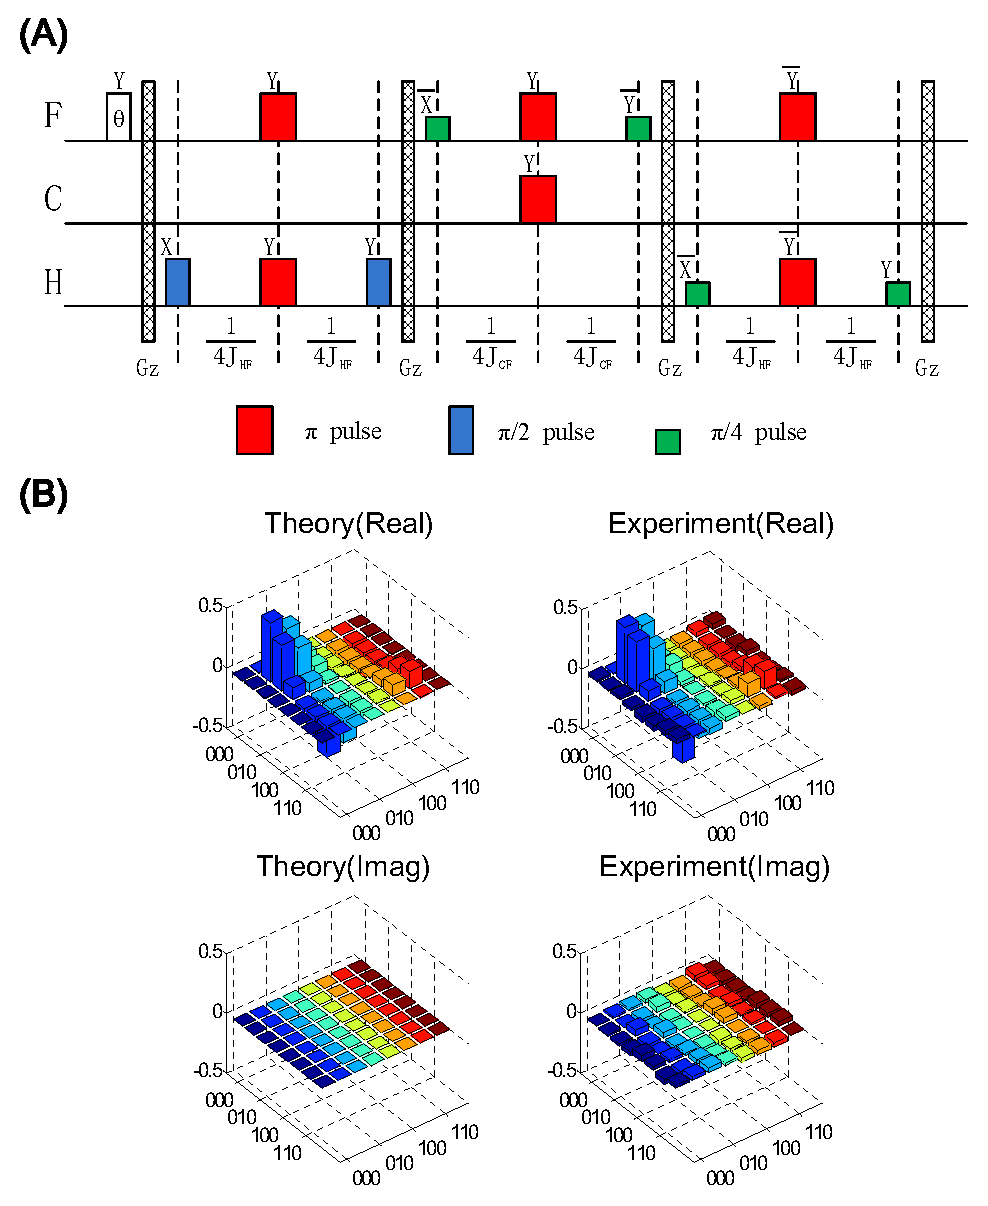
\includegraphics[width= 0.95\columnwidth]{pps.eps}
%\end{minipage}%
%\hspace{.05\textwidth}
%\begin{minipage}[c]{.3\textwidth}
%\centering
\caption{\footnotesize{(Color online) Pulse sequence for the preparation of the PPS and a comparison between experimental and theoretical density matrix elements for the reactant state $\left\vert \phi_{0} \right\rangle$.
(A) Pulse sequence that implements the PPS preparation, with $\theta=0.64\pi$ and $\texttt{X}(\overline{\texttt{X}}, \texttt{Y}, \overline{\texttt{Y}})$ representing rotations around the $x$($-x$, $y$, $-y$) direction. G$_\text{Z}$ represents a gradient pulse to destroy the coherence induced by
  the rotating pulses and free evolutions. $\frac{1}{4\text{J}_{\text{HF}}}$ and $\frac{1}{4\text{J}_{\text{CF}}}$ represent the free evolution of the system under $\mathcal{H}_{int}$ for 5.252 ms and 1.286 ms, respectively.
(B) Comparison between measured density matrix elements of the initial state $\left\vert \phi_{0} \right\rangle$ and the theoretial target density matrix elements based on the 8-point encoding. Both the real part and the imaginary part of the density matrix elements are shown.}}
\label{pps}
%\end{minipage}
\end{figure}


 The pulse sequence to prepare the PPS from the thermal equilibrium state is shown in Fig.~1(A). In particular,
 the gradient pulses (represented by G$_\text{Z}$) destroys the coherence induced by the rotating pulses and free evolutions. After obtaining the PPS,
 we apply one shaped pulse calculated by the GRadient Ascent Pulse Engineering (GRAPE) algorithm \cite{grape1-2,grape2-2,grape3-2} to obtain the initial state $\left\vert \phi_{0} \right\rangle$, with the pulse width 10 ms and a fidelity 0.995 (more GRAPE pulse information later). In order to assess the accuracy of the experimental preparation of the initial state, a full state tomography \cite{tomography} is implemented. The fidelity \cite{fidelity} between the target density matrix $\rho_{target}$ and the experimental density matrix $\rho_{exp}$ is found to be
\begin{eqnarray}\label{pps}
F(\rho_{target}, \rho_{exp})&\equiv& \texttt{Tr}(\rho_{target}\rho_{exp})/\sqrt{(\texttt{Tr}(\rho_{target}^2)\texttt{Tr}(\rho_{exp}^2)} \nonumber \\
&\approx & 0.95.
\end{eqnarray}
A detailed comparison between $\rho_{target}$ and $\rho_{exp}$ is displayed in Fig.~1(B).

\subsubsection*{\textbf{B. Dynamical Evolution}}

To observe the continuous reactant-to-product transformation, we divide the whole time evolution into 25 discrete steps. For convenience
all variables here are expressed in terms of atomic units.  For example, in atomic units $e=1$, $\hbar=1$, and $\delta t  = 62.02$.
  To exploit the split-operator scheme in Eq. (\ref{sop}), we let $H_0=T$, and $H'(t)=V-eq\epsilon(t)$.  The kinetic energy operator $T$ is diagonal in the momentum representation, whereas the $V$ operator and the dipole-field interaction $-eq\epsilon(t)$ operator are both diagonal in the position representation.  We then obtain from Eq. (\ref{sop})
\begin{eqnarray}
 U(t_m,t_{m-1})\approx  V_{\frac{\delta t}{2}}E_{\frac{\delta t}{2}}U_{QFT}T_{\delta t}U_{QFT}^{\dagger}E_{\frac{\delta t}{2}}V_{\frac{\delta t}{2}},
 \end{eqnarray}
where the operators
\begin{eqnarray}\label{potential}
V_{\frac{\delta t}{2}} &\equiv &e^{-i {V}\frac{\delta t}{2}},\\
T_{\delta t} &\equiv &e^{-i  {T}\delta t},\\
E_{\frac{\delta t}{2}} &\equiv&e^{i {q}\varepsilon(t_{m-1}+\delta t/2)\frac{\delta t}{2}}
\end{eqnarray}
are assumed to be in their diagonal representations.

To map $U(t_m,t_{m-1})$ to our 3-qubit NMR quantum computer, we discretize the potential energy curve using 8 grid points. Upon this discretization,
operators $V_{\frac{\delta t}{2}}$, $T_{\delta t}$, and $q$ become $8\times 8$ diagonal matrices. Numerically,  their diagonal elements  (denoted
$V_{diag}$, $T_{diag}$, and $q_{diag}$, respectively) are found to be
\begin{eqnarray}\label{operator}
  {V}_{diag} =&&(293.78,-0.10,1.85,5.41,\nonumber\\
             &&  5.46,2.02,0.18,305.44)\times 10^{-3};\nonumber\\
  {T}_{diag} =&&(0,0.91,3.63,8.16,\nonumber\\
&&  14.51,8.16,3.63,-0.91)\times 10^{-3};\nonumber\\
  {q}_{diag} =&&(-1.51,-1.08,-0.65,-0.22,\nonumber\\
&&  0.22,0.65,1.08,1.51).
\end{eqnarray}
To evaluate the $E_{\frac{\delta t}{2}}$ operator, we also need to discretize the time-dependence of the electric field associated with the ultrashort laser pulse.  For 25 snapshots of the reaction dynamics, we discretize the trapezoid-type electric field by 25 points, i.e., \begin{equation}\label{varepsilon}
\varepsilon(t)=[0.05,0.42,0.85,1,...1,0.85,0.42,0.05] \times 10^{-3}.
\end{equation}



The quantum gate network for the QFT operation that transforms the momentum representation to the coordinate representation is shown in Fig.~2. It consists of three Hardmard gates (H), three controlled-phase gates (S and T) and one SWAP gate (vertical line linking crosses).
The Hardmard gate H is represented by the Hardmard matrix
\begin{eqnarray}\label{Hardmard}
H = \frac{1}{\sqrt{2}}\left(
  \begin{array}{cc}
    1 & 1 \\
    1 & -1 \\
  \end{array}
\right),
\end{eqnarray}
which maps the basis state $\left\vert 0 \right\rangle$ to $\frac{1}{\sqrt{2}}(\left\vert 0 \right\rangle+\left\vert 1 \right\rangle)$ and $\left\vert 1 \right\rangle$ to $\frac{1}{\sqrt{2}}(\left\vert 0 \right\rangle-\left\vert 1 \right\rangle)$. The phase gates S and T are given by
\begin{eqnarray}\label{phasegate}
\text{S} = \left(
  \begin{array}{cc}
    1 & 0 \\
    0 & i \\
  \end{array}
\right)
\end{eqnarray}
and
\begin{eqnarray}\label{phasegate}
\text{T} = \left(
  \begin{array}{cc}
    1 & 0 \\
    0 & e^{i\pi/4} \\
  \end{array}
\right).
\end{eqnarray}
The matrix form of the SWAP gate is
\begin{eqnarray}\label{SWAP}
\text{SWAP} = \left(
         \begin{array}{cccc}
           1 & 0 & 0 & 0 \\
           0 & 0 & 1 & 0 \\
           0 & 1 & 0 & 0 \\
           0 & 0 & 0 & 1 \\
         \end{array}
       \right),
\end{eqnarray}
which exchanges the state of the $^{19}$F qubit and with that of the $^1$H qubit.

\begin{figure}[h]
%\centering
%\begin{minipage}[c]{.6\textwidth}
%\centering
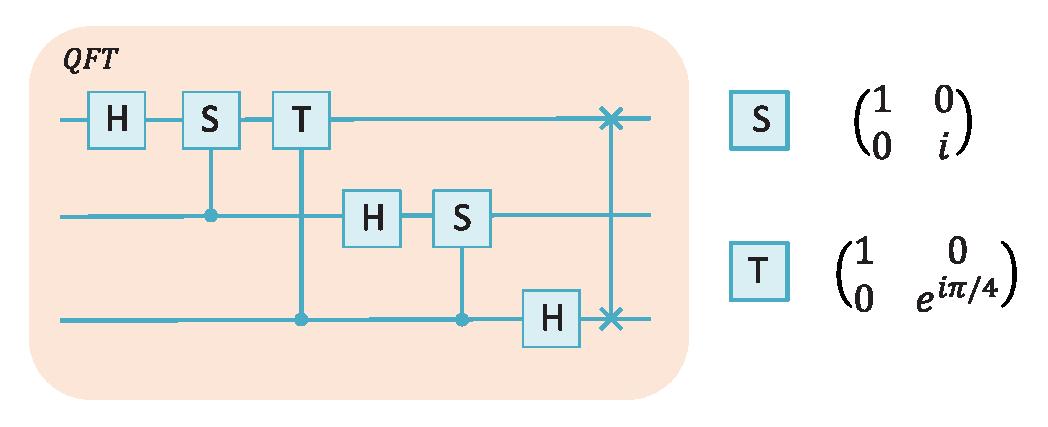
\includegraphics[width= 0.95\columnwidth]{qft.eps}
%\end{minipage}%
%\hspace{.05\textwidth}
%\begin{minipage}[c]{.3\textwidth}
%\centering
\caption{\footnotesize{(Color online) Network of implementing the QFT. H is the Hadamard gate and S, T are phase gates as specified on the right. Vertical lines ending with a solid dot represent controlled phase gates and the
vertical line between two crosses represents a SWAP gate.}}
\label{qft}
%\end{minipage}
\end{figure}

{\it GRAPE Pulses.} Since there are hundreds of logical gates in the required network of quantum operations, a direct implementation of the gate operation network will need a large number of single-qubit rotations as well as many free evolutions during the single-qubit operations. This bottom-up approach will
then accumulate the errors in every single-qubit operation. Considerable decoherence effects will also emerge during the long process. For example,
we have attempted to directly decompose the network into a sequence of RF pulses, finding that the required free evolution time for the 25 loops of evolution is more than 1 s, which is comparable to the $T_2$ time of our system.
To overcome these problems and to reach a high-fidelity quantum coherent control over the three interacting qubits, the unitary operators used in our experiment are realized by shaped quantum control pulses found by the GRadient Ascent Pulse Engineering (GRAPE) technique \cite{grape1-2,grape2-2,grape3-2}.
To maximize the fidelity of the experimental propagator as compared with the ideal gate operations, we use a mean gate fidelity by averaging over a weighted distribution of RF field strengths to minimize the inhomogeneity effect of the RF pulses applied to the sample.

For a known or desired unitary operator $U_{target}$,
the goal of the GRAPE algorithm is to find a shaped pulse within a given duration $t_{total}$ to maximize the fidelity
\begin{equation}\label{grape_fid}
F =|\texttt{Tr}(U_{target}^{\dagger}U_{cal})/2^n|^2,
\end{equation}
where $U_{cal}$ is the unitary operator actually realized by the shaped pulse and $2^n$ is the dimension of the Hilbert space. We discretize the evolution time $t_{total}$ into $N$ segments of equal duration $\Delta t = t_{total}/N$, such that $U_{cal}=U_N\cdots U_2U_1$, with the evolution operator associated with the \emph{j}th time interval given by
\begin{equation}
U_j=\exp\{-i\Delta t(\mathcal{H}_{int}+\sum_{k=1}^m u_k(j)\mathcal{H}_{k})\}.
\end{equation}
Here $\mathcal{H}_{int}$ is the three-qubit self-Hamiltonian in the absence of any control field, $\mathcal{H}_{k}$ represents the interaction Hamiltonians due to the applied RF field, and $u_k(j)$ is the control vectors associated with $\mathcal{H}_{k}$. Specifically, in our experiment $u_k(j)$ are the time-dependent amplitudes of the RF field along the \emph{x} and \emph{y} directions, for the F-channel, the C-channel and the H-channel.  With an initial guess for the pulse shape, we use the GRAPE algorithm to optimize $u_k(j)$ iteratively until $U_{cal}$ becomes very close to $U_{target}$.  More details can be found from Ref. \cite{grape1-2}. The GRAPE technique dramatically decreases the duration and complexity of our experiment and at the same time increases the quantum control fidelity.  In our proof-of-principle demonstration of the feasibility of the quantum simulation of a chemical reaction, the task of searching for the GRAPE pulses is carried out on a classical computer in a rather straightforward manner. It is important to note that this technique may be scaled up for many-qubit systems, because the quantum evolution of the system itself can be exploited in finding the high-fidelity coherent control pulses.


\begin{figure}[h]
%\centering
%\begin{minipage}[c]{.6\textwidth}
%\centering
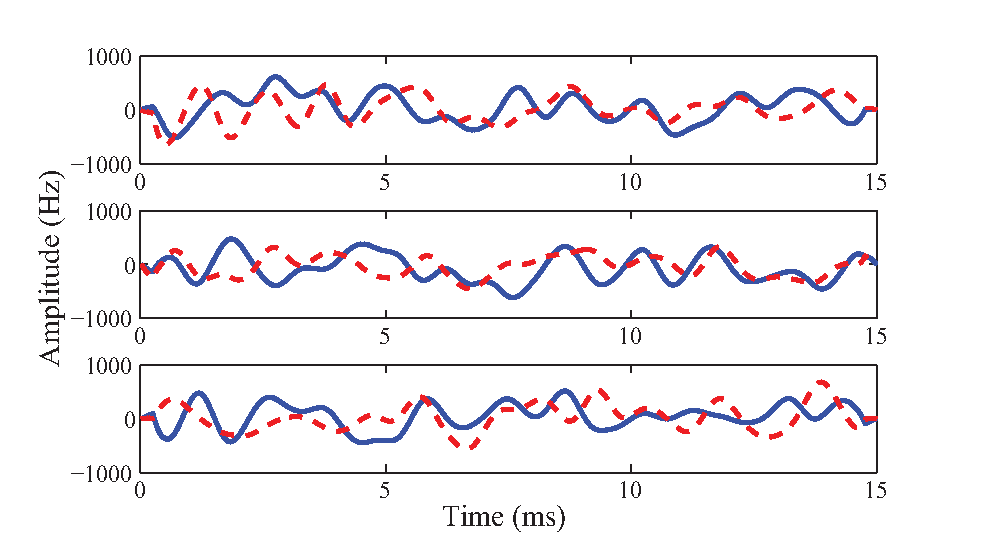
\includegraphics[width= 0.95\columnwidth]{grape.eps}
%\end{minipage}%
%\hspace{.05\textwidth}
%\begin{minipage}[c]{.3\textwidth}
%\centering
\caption{\footnotesize{(Color online) GRAPE pulse to simulate the quantum evolution of the reacting system from $t=0$ to $t_7=7\delta t$.
The top, middle and bottom panels depict the time-dependence of the RF pulses applied to the F-channel, C-channel and H-channel, respectively.
The (blue) solid line represents the pulse power applied in the ${x}$-direction, and the (red) dotted line represents the pulse power applied in the ${y}$-direction.}}
\label{grape}
%\end{minipage}
\end{figure}

%With all the operators confirmed, we can achieve any step of dynamical evolution theoretically. In experiment, since the direct decomposition would induct %very long and complicated pulse sequences, we utilized the GRAPE technique to pack the loops together to implement the desired operator, instead of %traditional decomposition of the network.
As an example,  Fig.~\ref{grape} shows the details of one 15 ms GRAPE pulse to realize the quantum evolution from $t=0$ to $t_7=7\delta t$ (also combining the operations for initial state preparation and the extra operation $R$ that is useful for the measurement stage). The shown GRAPE pulse is found by optimizing the frequency spectrum divided into 750 segments. The shown GRAPE pulse has a fidelity over 0.99.

\subsubsection*{\textbf{C. Measurement}}

To simulate the process of a chemical reaction, it is necessary to measure the simulated reactant-to-product transformation at different times. To that end we measure the overlaps of $C(\left\vert \psi({t_m}) \right\rangle,\left\vert \phi_{0} \right\rangle)$ and $C(\left\vert \psi(t_{m}) \right\rangle,\left\vert \phi_{1} \right\rangle)$ at $t_m=m\delta t$.
Here we first provide more explanations about how a diagonalization method can reduce the measurement of the overlaps to population measurements.


Without loss of generality, we consider the measurement $C(\left\vert \psi_{7} \right\rangle,\left\vert \phi_{0} \right\rangle)$.
\begin{equation}\label{overlap7}
C(\left\vert \psi(t_{7}) \right\rangle,\left\vert \phi_{0} \right\rangle)=| \la\phi_0|\psi(t_7)\ra |^2=\texttt{Tr}[\rho(t_7) \rho_0],
\end{equation}
where $\rho(t_7)=\left\vert \psi(t_{7} \right\rangle\left\langle \psi(t_{7}) \right\vert$ and $\rho_0=\left\vert \phi_{0} \right\rangle\left\langle \phi_{0} \right\vert$. Let \emph{R} be a transformation matrix which diagonalizes $\rho_0$ to a diagonal density matrix $\rho_0'=R \rho_0R^{\dagger}$. Then
\begin{eqnarray}\label{diag}
\texttt{Tr}[\rho(t_7) \rho_0]=\texttt{Tr}[R\rho(t_7) R^{\dagger}R \rho_0R^{\dagger}]=\texttt{Tr}[\rho'(t_7) \rho_0'],
\end{eqnarray}
where $\rho'(t_7)=R \rho(t_7)R^{\dagger}$.
Clearly then, only the diagonal terms (populations) of $\rho'(t_7)$ are relevant when calculating $\texttt{Tr}[\rho'(t_7) \rho_0']$,
namely, the overlap $C(\left\vert \psi(t_{7} \right\rangle,\left\vert \phi_{0} \right\rangle)$. Hence only population measurement of the  density matrix $\rho'(t_7)$ is needed to obtain the overlap between $|\psi(t_7)\rangle$ and the initial state.
The GRAPE pulse that combines the operations for initial state preparation, for the quantum evolution, as well as for the extra operation \emph{R} is already shown in Fig.~\ref{grape}.

\begin{figure}[h]
%\centering
%\begin{minipage}[c]{.6\textwidth}
%\centering
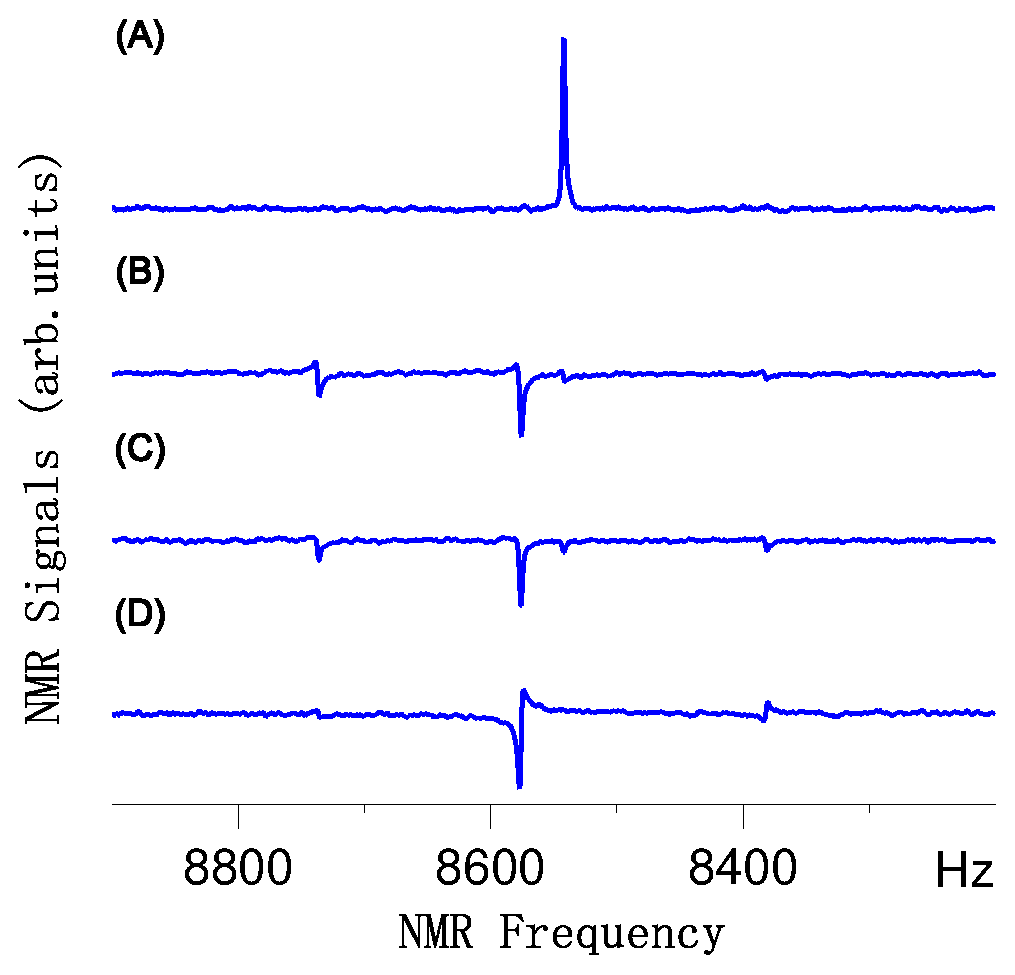
\includegraphics[width=0.95\columnwidth]{signal.eps}
%\end{minipage}%
%\hspace{.05\textwidth}
%\begin{minipage}[c]{.3\textwidth}
\centering
\caption{\footnotesize{(Color online) Measured spectra to extract the populations of the system density matrix before or after applying the GRAPE shown in Fig.~\ref{grape}.
(A) $^{13}$C spectrum of the PPS $\left\vert 000 \right\rangle$ as a result of a $[\pi/2]_y$ pulse applied to the $^{13}$C qubit.
The area (integral) of the absorption peak can be regarded as one benchmark in NMR realizations of
quantum computation. (B)-(D) Signals from the $^{19}$F, $^{13}$C and $^1$H qubits after applying the GRAPE pulse and a $[\pi/2]_y$ pulse to each of the three qubits. All the spectra are exhibited on the $^{13}$C channel through SWAP gates. The integration of each spectral peak gives the difference of two particular diagonal elements of the density matrix $\rho'(t_7)$.}}
\label{signal}
%\end{minipage}
\end{figure}

 The three population-readout spectra after applying the GRAPE pulse
 are shown in Fig.~\ref{signal}(B)-\ref{signal}(D), together with the $^{13}$C spectrum for the PPS $|000\rangle$.
 The populations to be measured are converted to the observable coherent terms by applying a $[\pi/2]_y$ pulse to each of the three qubits.   For the $^{13}$C spectrum shown in Fig.~\ref{signal}(C), four peaks from left to right are seen, with their respective integration results representing $P(5)-P(7)$, $P(6)-P(8)$, $P(1)-P(3)$, and $P(2)-P(4)$, where $P(i)$ is the  \emph{i}th diagonal element of $\rho'(t_7)$.  Experimentally the four integrals associated with the four peaks in Fig.~\ref{signal}(C) are found to be $-0.098$, $-0.482$, $-0.089$ and $-0.071$, which are close to the theoretical values $-0.047$, $-0.501$, $-0.114$ and $-0.041$.
 Further using other readouts from the $^{19}$F [see Fig.~\ref{signal}(B)] and $^1$H [see Fig.~\ref{signal}(D)] spectra as well as the normalization condition $\sum_{i=1}^{8} {P}({i})=1$, we obtain all the 8 populations and hence the overlap $C(\left\vert \psi(t_{7} \right\rangle,\left\vert \phi_{0} \right\rangle)$.  The theoretical and experimental results for this overlap are 0.535 and 0.529, which are in agreement.
 A similar procedure is used to obtain $C(\left\vert \psi(t_{m} \right\rangle,\left\vert \phi_{1} \right\rangle)$.

 The spectra of the ${}^{1}$H and ${}^{19}$F channel are obtained by first transmitting the signals of the $^{19}$F and $^1$H qubits to the $^{13}$C qubit using SWAP gates. With this procedure all the spectra shown in Fig.~\ref{signal} are exhibited on the $^{13}$C channel.  Indeed, because
 in our sample of natural abundance, only $\approx 1\%$ of all the molecules contain a ${}^{13}$C nuclear spin,
 the signals from the ${}^{1}$H and ${}^{19}$F nuclear spins  without applying SWAP gates would be
  dominated by those molecules with the ${}^{12}$C isotope.




\begin{thebibliography}{99}
\bibitem{Feynman2} R. P. Feynman, Rev. Mod. Phys. \textbf{20}, 367 (1948).
\bibitem{Feit2} M. D. Feit, J. A. Fleck, and A. Steiger, J. Comput. Phys. \textbf{47}, 412 (1982).
\bibitem{Kosloff} C. Leforestier \emph{et al}., J. Comput. Phys. \textbf{94}, 59 (1991).
\bibitem{Zhangbook2} J. Z. H. Zhang, {\it Theory and Application of Quantum Molecular Dynamics}
 (World Scientific, Singapore, 1999).
 \bibitem{bandrauk}A. D. Bandrauk and H. Chen, Can. J. Chem. {\bf 70}, 555 (1992).
 \bibitem{zhu}W. S. Zhu and X. S. Zhao, J. Chem. Phys. {\bf 105}, 9536 (1996).
\bibitem{spatial-2} D. G. Cory, A. F. Fahmy and T. F. Havel, Proc. Natl. Acad. Sci. USA. \textbf{94}, 1634 (1997).
\bibitem{grape1-2} N. Khaneja \emph{et al.}, J. Magn. Reson. \textbf{172}, 296 (2005).
\bibitem{grape2-2} J. Baugh \emph{et al.}, Phys. in Can. \textbf{63}, No.4
(2007).
\bibitem{grape3-2} C. A. Ryan \emph{et al.}, Phys. Rev. A \textbf{78}, 012328 (2008).
\bibitem{tomography} J. S. Lee, Phys. Lett. A \textbf{305}, 349 (2002).
\bibitem{fidelity} N. Boulant \emph{et al}., Phys. Rev. A \textbf{65}, 024302 (2002).
\end{thebibliography}



\end{document}




















